\chapter{Livro de Receitas}

\section{Mostrando Diálogos}

No Android podemos criar diálogos no \texttt{Activity} mostrando opções ao usuário, como por exemplo,
escolher itens de uma lista, ou responder sim ou não a uma ação, etc.

Vamos incrementar algumas partes de nosso código e tentar encaixar algumas funcionalidades
relacionadas.

\subsection{Editar/Excluir ao clicar e segurar na ListView}

Vamos implementar uma ação comum no mundo Android, que ao clicar e segurar num item
da \texttt{ListView}, ele mostra opções editar e excluir, por exemplo. Isto pode ser
feito facilmente usando \texttt{AlertDialog.Builder}, uma classe com métodos pré-prontos
para serem usados por você.

Neste exemplo precisaremos editar \texttt{ContatoHelper} e adicionar um método para
deletar um contato, editar nosso \texttt{MainActivity} no método \inlinecode{configurar}
e adicionar um \textit{Listener} que ao clicar e segurar num item da \texttt{ListView}
um método é acionado. Vamos a implementação:

% ContatoHelper.java
\begin{listing}[H]
  \inputminted[linenos=true,frame=bottomline,tabsize=3]{ java }{ source/ContatoHelper-5.java }
  \caption{Deletar dados existentes [ContatoHelper.java]}
\end{listing}

% MainActivity.java
\begin{listing}[H]
  \inputminted[linenos=true,frame=bottomline,tabsize=3]{ java }{ source/MainActivity-8.java }
  \caption{Adicionar Listener para click longo [MainActivity.java]}
\end{listing}

Note a necessidade de um novo método em \texttt{MainActivity}, o \inlinecode{exibirMensagem}.
Ele é bastante útil quando se quer exibir uma mensagem rapidamente e depois ela suma.
Para isso usamos a classe \texttt{Toast}.

\subsection{Diálogo de confirmação}

Deletar algo é uma coisa que deve ser feita com cuidado, então sempre é bom confirmar com
o usuário se ele deseja realmente deletar um contato. Para isso usaremos o \texttt{AlertDialog.Builder}
mais uma vez, agora apenas com uma mensagem e os botões \textit{Sim} ou \textit{Não}.


Ainda em \texttt{MainActivity} criaremos um outro \texttt{AlertDialog.Builder} no momento que o usuário
clicar em \texttt{Deletar}. Segue o trecho:

% MainActivity.java
\begin{listing}[H]
  \inputminted[linenos=true,frame=bottomline,tabsize=3]{ java }{ source/MainActivity-9.java }
  \caption{Diálogo de confirmação ao deletar contato [MainActivity.java]}
\end{listing}

Pronto, agora o trecho que deleta o contato foi movido para dentro do \textit{Listener} do botão
\textit{Sim}. No botão \textit{Não} passamos \texttt{null} no \textit{Listener}, pois caso
seja a opção escolhida apenas fazemos nada. Você pode se quiser criar um \textit{Listener} e mostrar
uma mensagem do tipo, \textit{Cancelado pelo usuário}, para isso usando o método \inlinecode{exibirMensagem}.

% DONE: fazer validação do telefone e do e-mail

\subsection{Entrada de diferentes tipos de dados}

O Android foi desenvolvido com muitos recursos pré-prontos para facilitar o desenvolvimento de aplicações.
Um recurso bastante útil é a distinção dos dados que irão ser inseridos nos \texttt{TextView}'s. Com isso
o teclado virtual do cliente se adapta ao tipo de dado que será inserido. No nosso caso faremos distinção
do campo \texttt{telefone}, onde apenas números e hífens(-) podem ser inseridos, e o campo \texttt{e-mail}
onde a presença do arroba(@) e pontos(.) são elementos essenciais.

Vejamos alguns valores aceitos pelo \texttt{inputType}:

\begin{itemize}

  \item Para textos:
  \begin{itemize}
    \item text
    \item textCapCharacters
    \item textMultiLine
    \item textUri
    \item textEmailAddress
    \item textPersonName
    \item textPassword
    \item textVisiblePassword
  \end{itemize}

  \item Para números:
  \begin{itemize}
    \item number
    \item numberSigned
    \item numberDecimal
    \item phone
    \item datetime
    \item date
    \item time
  \end{itemize}

\end{itemize}

Precisaremos alterar apenas o \texttt{salvar.xml} localizado em \texttt{res/layout}. Localize o atributo
\texttt{inputType} dos campos \texttt{telefone} e \texttt{e-mail} e altere os valores da seguinte maneira:

% res/layout/salvar.xml
\begin{listing}[H]
  \inputminted[linenos=true,frame=bottomline,tabsize=3]{ xml }{ source/salvar-2.xml }
  \caption{Distinção de dados [res/layout/salvar.xml]}
\end{listing}

\subsection{Validação de dados}

Mesmo configurando um \texttt{inputType} para seu \texttt{TextView} pode não ser o bastante para que
os dados inseridos estejam corretos. Para isso usaremos a classe \texttt{Patterns} do pacote
\texttt{android.util}. Nela podemos encontrar alguns objetos bastante úteis na hora de validar
dados. Entre eles estão os objetos \texttt{Patterns.EMAIL\b{ }ADDRESS} e \texttt{Patterns.PHONE}. Com
eles podemos validar de forma simples os dados inseridos em nosso formulário.

Em nosso \texttt{SalvarActivity} adicionaremos um método \inlinecode{validar} passando como parâmetro
um \texttt{Contato}. Copie o método \inlinecode{exibirMensagem} da classe \texttt{MainActivity} para
mostrar uma mensagem caso alguma validação seja falsa.

\paragraph{OBS:} Para um melhor reuso crie uma classe abstrata que implementa o método \inlinecode{exibirMensagem}
e que extenda de \texttt{Activity} e faça com que seus \texttt{Activity}'s herdem dela. É uma boa
prática.

Vamos ao trecho de código:

% SaveActivity.java
\begin{listing}[H]
  \inputminted[linenos=true,frame=bottomline,tabsize=3]{ java }{ source/SalvarActivity-4.java }
  \caption{Validação dos dados [SalvarActivity.java]}
\end{listing}

% DONE: fazer com que ao clicar e segurar fazer uma chamada ou enviar e-mail para o contato.
\subsection{Fazendo uma ligação}

Já que estamos fazendo uma lista de contatos nada melhor que usar o número do telefone dos
contatos inseridos para realizar chamadas. Para isso vamos aprender um pouco sobre \textbf{Permissões}.

Permissões no Android são definidas no \texttt{AndroidManifest.xml}. Ao instalar seu aplicativo,
o usuário saberá quais as permissões que o seu aplicativo necessita para ser executado.

Por padrão, o Android traz uma série de permissões que auxiliam seu aplicativo a se comunicar com
o aparelho. Abaixo alguns exemplos:

\begin{itemize}
\item Verificação
\begin{itemize}
  \item \texttt{ACCESS\b{ }NETWORK\b{ }STATE}
  \item \texttt{ACCESS\b{ }WIFI\b{ }STATE}
  \item \texttt{BATTERY\b{ }STATS}
\end{itemize}

\item Comunicação
\begin{itemize}
  \item \texttt{BLUETOOTH}
  \item \texttt{CALL\b{ }PHONE}
  \item \texttt{INTERNET}
  \item \texttt{SEND\b{ }SMS}
\end{itemize}

\end{itemize}

A lista completa pode ser vista em 
\url{http://developer.android.com/reference/android/Manifest.permission.html}.\\

Edite o \texttt{AndroidManifest.xml} e adicione a permissao \texttt{CALL\b{ }PHONE}.

% AndroidManifest.xml
\begin{listing}[H]
  \inputminted[linenos=true,frame=bottomline,tabsize=3]{ xml }{ source/AndroidManifest-3.xml }
  \caption{Permissão de realizar chamadas [AndroidManifest.xml]}
\end{listing}

Agora vamos adicionar um item ao diálogo que aparece ao clicar e segurar um item da \texttt{ListView}.
Ele servirá para implementarmos o trecho que realiza a chamada. Vamos a ele:

% MainActivity.java
\begin{listing}[H]
  \inputminted[linenos=true,frame=bottomline,tabsize=3]{ java }{ source/MainActivity-10.java }
  \caption{Item chamar no diálogo [MainActivity.java]}
\end{listing}

\newpage

\subsection{Enviando e-mail}

Para envio de e-mail você pode simplesmente usar a aplicação de e-mail padrão do aparelho.
Seguindo o mesmo princípio do exemplo anterior vamos apenas inserir um trecho de código
no método \inlinecode{configurar} da classe \texttt{MainActivity}:

% MainActivity.java
\begin{listing}[H]
  \inputminted[linenos=true,frame=bottomline,tabsize=3]{ java }{ source/MainActivity-11.java }
  \caption{Item enviar e-mail no diálogo [MainActivity.java]}
\end{listing}

Ao testar no emulador você receberá a mensagem: \textbf{No applications can perform this action}. Traduzindo
quer dizer que: Nenhuma aplicação pode executar esta ação. Em outras palavras, nenhum cliente de e-mail
foi encontrado.
 
% protected void sendnotification (String title, String message) {
%    String ns = Context.NOTIFICATION_SERVICE;
%    NotificationManager mNotificationManager = (NotificationManager) getSystemService(ns);
%  
%    int icon = R.drawable.icon;
%    CharSequence tickerText = message;
%    long when = System.currentTimeMillis();
% 
%    Notification notification = new Notification(icon, tickerText, when);
% 
%    Context context = getApplicationContext();
%    CharSequence contentTitle = title;
%    CharSequence contentText = message;
%    Intent notificationIntent = new Intent(this, AndroToDo.class);
%    PendingIntent contentIntent = PendingIntent.getActivity(this, 0, notificationIntent, 0);
% 
%    notification.flags = Notification.FLAG_AUTO_CANCEL;
%    notification.setLatestEventInfo(context, contentTitle, contentText, contentIntent);
%    mNotificationManager.notify(NOTIFICATION_ID, notification);
% }
% // see http://androidsnippets.com/send-a-notification

\section{Internacionalização (i18n)}

\subsection{Forçando região para teste}

Para podermos testar as \texttt{strings} de i18n podemos forçar o \texttt{Activity}
a utilizar uma determinada linguagem. Isso se dá por meio da classe \texttt{Locale}.
Façamos um teste com o \texttt{SalvarActivity} inserindo o trecho de código abaixo no
método \texttt{onCreate}. Vamos a ele:

% SaveActivity.java
\begin{listing}[H]
  \inputminted[linenos=true,frame=bottomline,tabsize=3]{ java }{ source/SalvarActivity-5.java }
  \caption{Forçando região [SalvarActivity.java]}
\end{listing}

Para visualizar a mudança crie \textit{strings} no seu arquivo \texttt{strings.xml}. Substitua
as \textit{strings} \texttt{Nome}, \texttt{Telefone}, \texttt{E-mail} e \texttt{Salvar} pelos
respectivos valores em inglês \texttt{Name}, \texttt{Phone}, \texttt{E-mail} e \texttt{Save}.
Agora crie outro arquivo \texttt{strings.xml} dentro do diretório \texttt{/res/values-pt-rBR} e
insira as mesmas \textit{strings} citadas anteriormente, traduzindo cada valor.

Faça testes comentando a chamada para a função \texttt{forceLocale} e veja as mudanças.

\subsection{Forçando região pelo emulador}

A maneira mais rápida e prática de forçar a região é pelo próprio emulador. Vá até a lista de
aplicativos e procure por \texttt{Custom Locale}. Depois pesquise por \texttt{pt\b{ }BR} e caso não encontre
clique em \texttt{Add New Locale}. Digite \texttt{pt\b{ }BR} e clique em \texttt{Add and Select}.

% Preferencias
\section{Utilizando as Preferências do Android}

O Android já disponibiliza uma maneira de criar preferências de forma fácil. Para demostrar implementaremos
um exemplo bem amplo, que irá nos ajudar a entender ainda mais de Android. Para começar adicionaremos
um nova coluna a nossa tabela \texttt{contato} chamada \texttt{grupo}. Depois adicionaremos um \textit{array}
de \textit{string}'s ao nosso arquivo \texttt{strings.xml} e ainda vamos aprender a utilizar um
\texttt{Spinner}, também conhecido como \textit{combo box}. Por último, e não menos importante, usaremos
as preferências para tornar padrão um valor de nosso \texttt{Spinner}.

% spinner: http://www.dcpagesapps.com/developer-resources/android/21-android-tutorial-spinners?start=2
% spinner, preferencias: http://www.dcpagesapps.com/developer-resources/android/23-android-spinner-tips?start=1

\subsection{Atualizando colunas de uma tabela}

Como visto em \ref{ssec:model}, a classe \texttt{SQLiteOpenHelper} obriga-nos a implementar os métodos
\inlinecode{onCreate} e \inlinecode{onUpgrade}. Neste ponto será necessário o uso do método \inlinecode{onUpgrade}.
Ele serve, como o nome sugere, para atualizar a \gls{ddl} do banco de dados. Isso é útil quando seu cliente
já possui uma versão do seu aplicativo instalada e ele quer apenas atualizar para uma nova versão. Também será
necessário adicionar a coluna \texttt{grupo} nas \textit{queries}. Abra a classe \texttt{ContatoHelper} em
\texttt{contatos.app.model} e faça as modificações:

% ContatoHelper.java
\begin{listing}[H]
  \inputminted[linenos=true,frame=bottomline,tabsize=3]{ java }{ source/ContatoHelper-6.java }
  \caption{Nova coluna grupo na base de dados [ContatoHelper.java]}
\end{listing}

Vemos neste exemplo o uso da classe \texttt{Log} do pacote \texttt{android.util}. Ela possui apenas
métodos estáticos, assim não precisamos instanciar, apenas faça a chamada dos métodos. Temos:
\begin{description}
\item[\inlinecode{Log.w()}] para mostrar \textit{warning}'s, ou seja, avisos.
\item[\inlinecode{Log.e()}] para mensagens de erro.
\item[\inlinecode{Log.d()}] para mensagens \textit{\gls{debug}}.
\item[\inlinecode{Log.i()}] para mensagens informativas.
\item[\inlinecode{Log.v()}] para outras mensagens.
\end{description}

% ContatoHelper.java
\begin{listing}[H]
  \inputminted[linenos=true,frame=bottomline,tabsize=3]{ java }{ source/ContatoHelper-7.java }
  \caption{Modificação nas queries [ContatoHelper.java]}
\end{listing}

\subsection{Array de Strings}

No arquivo de \textit{string}'s do Android é possível criar vários recursos. Dentre eles temos Cor,
Dimensão, Estilo/Tema. Usando a ferramenta ADT, crie um \texttt{String Array} em \texttt{strings.xml}
dentro de \texttt{res/values} e adicione alguns itens para representar os valores da coluna \texttt{grupo},
e outro \texttt{String Array} para representar os índices:

\paragraph{Dica:} você pode tentar implementar o trecho usando uma tabela do banco de dados. A ideia
é a mesma, neste caso não seria necessário o uso de \texttt{String Array}'s.

% strings.xml
\begin{listing}[H]
  \inputminted[linenos=true,frame=bottomline,tabsize=3]{ xml }{ source/strings-1.xml }
  \caption{Array de Strings [strings.xml]}
\end{listing}

\subsection{Spinner, diálogo de seleção}

O Spinner é ideal quando temos que escolher entre valores fixos, sejam eles estáticos ou dinâmicos.
Nosso exemplo irá utilizar valores estáticos para popular o mesmo. Para isso utilizaremos o
\texttt{array\b{ }grupos} que criamos em \texttt{res/values/strings.xml}. Também veremos um exemplo
de uso da classe \texttt{android.R} como visto em \ref{par:r} em que é explicado a diferença entre
as classes de recusros. Mas antes temos que atualizar nosso \textit{layout} \texttt{salvar.xml}.
Segue o trecho:

% res/layout/salvar.xml
\begin{listing}[H]
  \inputminted[linenos=true,frame=bottomline,tabsize=3]{ xml }{ source/salvar-3.xml }
  \caption{Adicionando elemento Spinner [res/layout/salvar.xml]}
\end{listing}

Adicione o Spinner logo abaixo do \texttt{e-mail}. Agora já podemos carregar e popular o Spinner
na classe \texttt{SalvarActivity}.

% SaveActivity.java
\begin{listing}[H]
  \inputminted[linenos=true,frame=bottomline,tabsize=3]{ java }{ source/SalvarActivity-6.java }
  \caption{Utilização de Spinner [SalvarActivity.java]}
\end{listing}

Note a utilização da classe \texttt{android.R} nas linhas \circled{10} e \circled{11}. Eles servem
para definir o \textit{layout} do Spinner. Isso quer dizer que você pode implementar como seu Spinner
irá aparecer na tela da mesma maneira que implementamos a linha da \texttt{ListView} em \ref{ssec:listview}.

\subsection{A classe PreferenceActivity}

Afinal vamos utilizar as preferências do Android. Neste exemplo a usaremos para decidir qual grupo
do \texttt{array\b{ }grupos} aparecerá selecionado por padrão. A princípio é um exemplo bem simples, mas
que pode ser ajustado para outras finalidades, o que importa realmente é a ideia.

Para começar criaremos um \textit{layout} em \texttt{res/layout} chamado \texttt{preferencias.xml}.
No projeto clique com botão direito do \textit{mouse} e selecione \texttt{New $\rightarrow$ Other...},
pesquise por \texttt{Android XML File} e \texttt{Next}. Em \texttt{Resource Type} escolha
\texttt{Preference} e escreva \texttt{preferencias} em \texttt{File}. Logo abaixo em \texttt{Root Element}
escolha a opção \texttt{PreferenceScreen}, então \texttt{Finish}.

Utilizando a ferramenta ADT adicione um elemento \texttt{ListPreference} a \texttt{PreferenceScreen}.
Defina os parâmetros necessários como mostra o código abaixo:

% preferencias.xml
\begin{listing}[H]
  \inputminted[linenos=true,frame=bottomline,tabsize=3]{ xml }{ source/preferencias-1.xml }
  \caption{XML descrevendo layout de preferências [res/xml/preferencias.xml]}
\end{listing}

Crie uma nova classe chamada \texttt{EditarPreferencias} em \texttt{contatos.app.view} herdando de
\texttt{PreferenceActivity}. Agora de uma maneira bem simples implementaremos essa classe. Veja:

% EditarPreferencias.java
\begin{listing}[H]
  \inputminted[linenos=true,frame=bottomline,tabsize=3]{ java }{ source/EditarPreferencias-1.java }
  \caption{Activity para mostrar preferências [EditarPreferencias.java]}
\end{listing}

Para chamar a nova \texttt{Activity} temos ainda que mapeá-la no \texttt{AndroidManifest} e criar
um item no menu.

% AndroidManifest.xml
\begin{listing}[H]
  \inputminted[linenos=true,frame=bottomline,tabsize=3]{ xml }{ source/AndroidManifest-4.xml }
  \caption{Mapeando Activity EditarPreferencias [AndroidManifest.xml]}
\end{listing}

% res/menu/main_menu.xml
\begin{listing}[H]
  \inputminted[linenos=true,frame=bottomline,tabsize=3]{ xml }{ source/main_menu-2.xml }
  \caption{Adicionar item Preferências ao menu principal [res/menu/main\b{ }menu.xml]}
\end{listing}

Agora que adicionamos um item ao menu, temos que capturar o evento quando o usuário o selecionar
e direcioná-lo as Preferências. Isso deve ser feito em \texttt{MainActivity}.

% MainActivity.java
\begin{listing}[H]
  \inputminted[linenos=true,frame=bottomline,tabsize=3]{ java }{ source/MainActivity-12.java }
  \caption{Ir para Preferências pelo menu principal [MainActivity.java]}
\end{listing}

Note que para ter um código mais eficiente e otimizado tivemos que mudar o método \inlinecode{irParaSalvar}
para \inlinecode{irPara} passando como parâmetro a classe que desejamos ir. Essa mudança é boa mais causa
um impacto em outros trechos do código. Conserte-os da seguinte maneira:

% MainActivity.java
\begin{listing}[H]
  \inputminted[linenos=true,frame=bottomline,tabsize=3]{ java }{ source/MainActivity-13.java }
  \caption{Mudança em método irParaSalvar [MainActivity.java]}
\end{listing}

Por fim temos que selecionar o tem que o usuário quer que esteja selecionado por padrão ao inserir
um novo contato. Assim, em \texttt{SalvarActivity} adicione o trecho:

% SaveActivity.java
\begin{listing}[H]
  \inputminted[linenos=true,frame=bottomline,tabsize=3]{ java }{ source/SalvarActivity-7.java }
  \caption{Obtem o valor padrão definido nas Preferências [SalvarActivity.java]}
\end{listing}

\section{Grupo de Contatos usando Grid}

Uma das coisas mais legais quando falamos de aparelhos móveis é a ideia da visão da lista de aplicativos
usada comumente com o ícone e o texto logo abaixo. Essa ideia pode ser facilmente implementada em
um aplicativo Android usando \texttt{GridView}.

Nessa implementação vamos criar uma tela que mostra os grupos de contatos em forma de \textit{Grid}
e ao clicar levaremos o usuário a lista de contatos mostrando apenas aqueles contatos do determinado
grupo.

\subsection{Layout usando GridView}

Para começar criaremos um \textit{layout} em \texttt{res/layout} chamado \texttt{grupos\b{ }item.xml}.
Ele irá conter a imagem e o texto que serão exibidos no \texttt{GridView}. Faça como mostra o trecho abaixo:

% res/layout/grupos_item.xml
\begin{listing}[H]
  \inputminted[linenos=true,frame=bottomline,tabsize=3]{ xml }{ source/grupos_item-1.xml }
  \caption{Item do Layout de Grupos [res/layout/grupos\b{ }item.xml]}
\end{listing}

Hora de criar o \texttt{GridView}. Para isso crie um novo \textit{layout} em \texttt{res/layout} chamado
\texttt{grupos.xml}. Adicione apenas um \texttt{GridView} como mostra o trecho de código abaixo:

% res/layout/grupos.xml
\begin{listing}[H]
  \inputminted[linenos=true,frame=bottomline,tabsize=3]{ xml }{ source/grupos-1.xml }
  \caption{Layout de Grupos [res/layout/grupos.xml]}
\end{listing}

\paragraph{Dica:} a ferramenta ADT provê uma forma de pré-visualizar seu \textit{layout}. Note que
na linha \circled{12} temos um comentário e nele temos a referência ao \textit{layout}
\texttt{grupos\b{ }item}. Para isso apenas clique com botão direito do \textit{mouse} na \texttt{GridView}
e na opção \texttt{Preview Grid Content $\rightarrow$ Choose Layout...} selecione \texttt{grupos\b{ }item}.

\subsection{Activity para visualizar os Grupos}

Como é de se imaginar temos que criar uma \texttt{Activity} para visualizar os Grupos.

% GruposActivity.java
\begin{listing}[H]
  \inputminted[linenos=true,frame=bottomline,tabsize=3]{ java }{ source/GruposActivity-1.java }
  \caption{Activity para visualizar Grupos [GruposActivity.java]}
\end{listing}

Temos que criar duas classes internas para nos ajudar a criar cada item do grupo de contatos.
Para isso usaremos a classe abstrata \texttt{BaseAdapter}.

% GruposActivity.java
\begin{listing}[H]
  \inputminted[linenos=true,frame=bottomline,tabsize=3]{ java }{ source/GruposActivity-2.java }
  \caption{Adapter responsável por cada item do Grid [GruposActivity.java]}
\end{listing}

Chegou a hora de você usar a ferramenta Inkscape e criar alguns ícones. Para os exemplos a seguir
você deve criar um ícone para cada item do grupo, sendo eles:

\begin{itemize}
	\item amigos
	\item trabalho
	\item conhecidos
	\item família
\end{itemize}

Para título de exemplo crie apenas ícones simples e depois tente fazer itens mais sofisticados. Em
\url{http://developer.android.com/design/style/iconography.html} você pode ver como devem ser criados
os ícones para seu aplicativo.

\subsubsection{Criando ícones com Inkscape}

Use o Inkscape para criar um novo ícone. No menu \texttt{Arquivo $\rightarrow$
Propriedades do Desenho...} ou apenas \texttt{Shift + Ctrl + D} e altere a largura e altura
para \texttt{512px}.

Aperte \texttt{5} para centralizar a folha e crie um quadrado (\texttt{F4}) um pouco menor que a página.
Utilize \texttt{Ctrl} para criar um quadrado perfeito. Altere a borda usando o círculo branco no canto
superior direito do quadrado. Selecione uma cor legal.

O Android possui uma paleta de cores que pode lhe ajudar inicialmente. Veja a tabela abaixo:

\begin{table}[H]
\begin{tabularx}{310pt}{Xcc}
\hline
\textbf{Cor} & \textbf{Tom claro} & \textbf{Tom escuro}\\
\hline
Azul & \texttt{\#33B5E5} \fcolorbox{black}{android-blue}{\textcolor{android-blue}{TTT}}
		& \texttt{\#0099CC} \fcolorbox{black}{android-dark-blue}{\textcolor{android-dark-blue}{TTT}}\\
Roxo & \texttt{\#AA66CC} \fcolorbox{black}{android-purple}{\textcolor{android-purple}{TTT}}
		& \texttt{\#9933CC} \fcolorbox{black}{android-dark-purple}{\textcolor{android-dark-purple}{TTT}}\\
Verde & \texttt{\#99CC00} \fcolorbox{black}{android-green}{\textcolor{android-green}{TTT}}
		& \texttt{\#669900} \fcolorbox{black}{android-dark-green}{\textcolor{android-dark-green}{TTT}}\\
Laranja & \texttt{\#FFBB33} \fcolorbox{black}{android-orange}{\textcolor{android-orange}{TTT}}
		& \texttt{\#FF8800} \fcolorbox{black}{android-dark-orange}{\textcolor{android-dark-orange}{TTT}}\\
Vermelho & \texttt{\#FF4444} \fcolorbox{black}{android-red}{\textcolor{android-red}{TTT}}
		& \texttt{\#CC0000} \fcolorbox{black}{android-dark-red}{\textcolor{android-dark-red}{TTT}}\\
\hline
\end{tabularx}
\caption{Paleta de cores do Android}
\end{table}

Mais detalhes em \url{http://developer.android.com/design/style/color.html}.

\bigskip

Para alterar a cor clique com botão direito do \textit{mouse} no quadrado e selecione
\texttt{Preenchimento e contorno}. Observe a entrada de texto onde aparece \texttt{RGBA}.
Altere com os valores acima mantendo os dois últimos, pois eles são referentes a transparência.

Chegou a hora de exportar seu ícone para os tamanhos sugeridos pelo Android. Basta ir no menu
\texttt{Arquivo $\rightarrow$ Exportar Bitmap...} ou ainda \texttt{Shift + Ctrl + E}. Os tamanhos
estão definidos na tabela abaixo:

\begin{table}[H]
\begin{tabularx}{300pt}{Xc}
\hline
\textbf{Local} & \textbf{Tamanho}\\
\hline
\texttt{res/drawable-xhdpi} & \texttt{96px}\\
\texttt{res/drawable-hdpi} & \texttt{72px}\\
\texttt{res/drawable-mdpi} & \texttt{48px}\\
\texttt{res/drawable-ldpi} & \texttt{36px}\\
\hline
\end{tabularx}
\caption{Paleta de cores do Android}
\end{table}

Exporte o ícone para cada um desses diretórios, crie-os caso não existam. Como temos quatro
grupos crie quatro ícones usando cores diferentes. Siga a nomenclatura sugerida em \ref{sssec:nomeicones}
Convenção de nomes para ícones, exemplo: \texttt{ic\b{ }launcher\b{ }grupo\b{ }amigos.png}.

\subsection{Implementando o Adapter}

% GruposActivity.java
\begin{listing}[H]
  \inputminted[linenos=true,frame=bottomline,tabsize=3]{ java }{ source/GruposActivity-3.java }
  \caption{implementação do Adapter [GruposActivity.java]}
\end{listing}

Como visto em \ref{ssec:listview} Mostrando os dados na View, no \texttt{Adapter} podemos fazer
\textit{cache} dos objetos e otimizar o código. Isso pode ser observado a partir da linha \circled{25}
até a linha \circled{35}, onde um teste é realizado para ver se a linha está em \textit{cache}.

\paragraph{Observação:} na linha \circled{37} existe um trecho de código que não está nada otimizado.
No entanto usando \texttt{string-array} é a única maneira de dar certo. Isso poderia ser evitado se
os grupos de contatos fossem retirados do banco de dados. Seguindo as instruções antes abordadas tente
você mesmo implementar usando banco de dados. É uma ótima maneira de aprender melhor como funciona
um aplicativo Android.

\medskip

Finalize adicionando o \texttt{Activity} no \texttt{AndroidManifest.xml}. Clique na aba inferior em
\texttt{Application} e em \texttt{Application Nodes} clique em \texttt{Add}. Escolha \texttt{Activity}
na lista de opções e no atributo \texttt{Name} clique em \texttt{Browser} e busque por
\texttt{GruposActivity}.

Para visualizar a nova \texttt{Activity} é preciso adicionar um novo item no menu principal. Reveja
\ref{ssec:act} Activity, e implemente essa parte. Não esqueça de adicionar uma condição no método
\inlinecode{onOptionsItemSelected} da classe \texttt{MainActivity}.

%  TODO: utilizar GruposActivity para mostrar apenas contatos de um determinado grupo.
%  TODO: colocar screenshot da tela de grupos

\subsection{Selecionando contatos de um determinado grupo}

Para não deixar dúvidas quanto a implementação deste trecho vamos fazer com que ao clicar
em um determinado grupo, somente contatos daquele grupo apareçam na lista que fica
em \texttt{MainActivity}.

Primeiro sobrescreva o método \inlinecode{listar} da classe \texttt{ContatoHelper} para que
ele receba um parâmetro, que irá representar o grupo.

% ContatoHelper.java
\begin{listing}[H]
  \inputminted[linenos=true,frame=bottomline,tabsize=3]{ java }{ source/ContatoHelper-8.java }
  \caption{Método listar com parâmetro grupo [ContatoHelper.java]}
\end{listing}

A implementação do clique em um item do \textit{grid} é semelhante a vista em \ref{ssec:edit}
Editando dados existentes, onde criamos uma variável contendo o \textit{namespace} do nosso parâmetro.

Copie o método \inlinecode{irPara} da classe \texttt{MainActivity}, mudando apenas o primeiro
parâmetro de \inlinecode{intent.putExtra} para o novo \textit{namespace}, na linha \circled{17}.

Por fim, inclua o método \inlinecode{configurar} em \inlinecode{onCreate}, o qual será responsável
por configurar para onde ir ao clicar em um item do \textit{grid}.

% GruposActivity.java
\begin{listing}[H]
  \inputminted[linenos=true,frame=bottomline,tabsize=3]{ java }{ source/GruposActivity-4.java }
  \caption{Evento de clique em um item do \textit{grid} [GruposActivity.java]}
\end{listing}

Agora é preciso capturar o parâmetro em \texttt{MainActivity}. Para isso basta fazer como descrito abaixo:

% MainActivity.java
\begin{listing}[H]
  \inputminted[linenos=true,frame=bottomline,tabsize=3]{ java }{ source/MainActivity-14.java }
  \caption{Captura de parâmetro vindo de \texttt{GruposActivity} [MainActivity.java]}
\end{listing}

Muito bem, eis que temos um aplicativo já bem completo. Se tudo deu certo você deve ter uma tela como
vemos abaixo:

\begin{figure}[h]
\centering
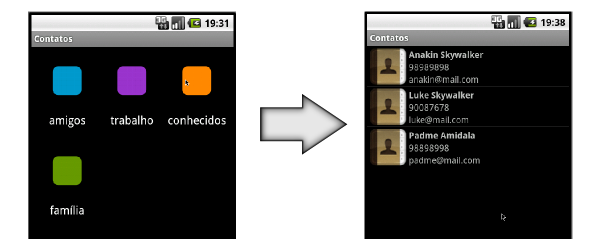
\includegraphics{img/screenshot-grupos.png}
\caption{Tela de Grupos}
\end{figure}